\documentclass{article}\usepackage[]{graphicx}\usepackage[]{color}
%% maxwidth is the original width if it is less than linewidth
%% otherwise use linewidth (to make sure the graphics do not exceed the margin)
\makeatletter
\def\maxwidth{ %
  \ifdim\Gin@nat@width>\linewidth
    \linewidth
  \else
    \Gin@nat@width
  \fi
}
\makeatother

\definecolor{fgcolor}{rgb}{0.345, 0.345, 0.345}
\newcommand{\hlnum}[1]{\textcolor[rgb]{0.686,0.059,0.569}{#1}}%
\newcommand{\hlstr}[1]{\textcolor[rgb]{0.192,0.494,0.8}{#1}}%
\newcommand{\hlcom}[1]{\textcolor[rgb]{0.678,0.584,0.686}{\textit{#1}}}%
\newcommand{\hlopt}[1]{\textcolor[rgb]{0,0,0}{#1}}%
\newcommand{\hlstd}[1]{\textcolor[rgb]{0.345,0.345,0.345}{#1}}%
\newcommand{\hlkwa}[1]{\textcolor[rgb]{0.161,0.373,0.58}{\textbf{#1}}}%
\newcommand{\hlkwb}[1]{\textcolor[rgb]{0.69,0.353,0.396}{#1}}%
\newcommand{\hlkwc}[1]{\textcolor[rgb]{0.333,0.667,0.333}{#1}}%
\newcommand{\hlkwd}[1]{\textcolor[rgb]{0.737,0.353,0.396}{\textbf{#1}}}%

\usepackage{framed}
\makeatletter
\newenvironment{kframe}{%
 \def\at@end@of@kframe{}%
 \ifinner\ifhmode%
  \def\at@end@of@kframe{\end{minipage}}%
  \begin{minipage}{\columnwidth}%
 \fi\fi%
 \def\FrameCommand##1{\hskip\@totalleftmargin \hskip-\fboxsep
 \colorbox{shadecolor}{##1}\hskip-\fboxsep
     % There is no \\@totalrightmargin, so:
     \hskip-\linewidth \hskip-\@totalleftmargin \hskip\columnwidth}%
 \MakeFramed {\advance\hsize-\width
   \@totalleftmargin\z@ \linewidth\hsize
   \@setminipage}}%
 {\par\unskip\endMakeFramed%
 \at@end@of@kframe}
\makeatother

\definecolor{shadecolor}{rgb}{.97, .97, .97}
\definecolor{messagecolor}{rgb}{0, 0, 0}
\definecolor{warningcolor}{rgb}{1, 0, 1}
\definecolor{errorcolor}{rgb}{1, 0, 0}
\newenvironment{knitrout}{}{} % an empty environment to be redefined in TeX

\usepackage{alltt}
\usepackage[top=1in,bottom=1in,left=1in,right=1in]{geometry}
\usepackage[colorlinks=true,allcolors=Blue]{hyperref}
\usepackage{cleveref}
\usepackage[usenames,dvipsnames]{xcolor}

% knitr options


\IfFileExists{upquote.sty}{\usepackage{upquote}}{}
\begin{document}

\setlength{\parskip}{5mm}
\setlength{\parindent}{0in}

\title{Simulation and removal of advection effects on DO measurements}
\author{Marcus W. Beck}
\maketitle

\section{Overview}

Observed DO in estuaries can be described as the summation of DO from biological processes, air-sea gas diffusion, water transport by tidal advection, and error or noise.  
\begin{equation} \label{eqn:one}
DO_{obs} = DO_{bio} + DO_{dif} + DO_{adv}
\end{equation}
Reliable estimates of ecosystem metabolism are dependent on measures of DO flux that are dominated by biological processes.  Long-term time series of DO measurements may include variation related to both biological and physical processses such that the use of observed data may be insufficient in many examples.  Statistical modelling techniques that quantify variation in DO over time and tidal changes have the potential to isolate biological signals in DO variation to more accurately estimate metabolism.  We used a simulation approach to create an observed DO time series as the summation of diel variation.  The effects of air-sea gas diffusion were not considered in the simulation given that methods for quantifying the contribution are available and not of concern for the analysis.  A weighted regression approach was used to predict the simulated time series and then remove variation related to tidal changes.  The following describes the general approach and results of the analysis.

First, a biological DO time series was created using a sine/cosine function where:

\begin{equation} \label{eqn:bio}
DO_{bio} = \alpha + \beta\cos\left(2\pi ft + \Phi\right)
\end{equation}

where the mean DO $\alpha$ was 8, amplitude $\beta$ was 1, $f$ was 1/48 to repeat on a 24 hour period (30 minute observations, \cref{fig:do_sim}), $t$ was the time series vector and $\Phi$ was the x-axis origin set for sunrise at 630am.  The signal was increasing during hypothetical daylight and decreasing during the night for each 24 hour period.  The signal ranged from 7 to 9 mg L$^{-1}$.

Noise was added to the biological DO signal to simulate natural variation in DO throughout the time series (\cref{fig:do_sim}).  Total uncertainty was the sum of process and observation uncertainty simulated as random variables from the normal distribution, such that:
\begin{equation}
\epsilon _{tot} = \epsilon _{obs} + \int_0^n \epsilon _{pro}
\end{equation}
where $\epsilon$ for observation and process uncertainty was simulated as a normally distributed random variable with mean zero and standard deviation varying from zero to an upper limit, described below.  The noise for process uncertainty was estimated as a cumulative sum for time $t$ in 0 to $n$ observations such that the noise at time $t+1$ was equal to the noise at time $t$ plus additional variation drawn from the normal distribution.  This approach created a noise vector that was auto-correlated throughout the time series.  The noise vector for process uncertainty was rescaled to constrain the variation within the bounds for standard deviation defined by the random variable. The total error was added to the biological DO time series and was assumed to represent variation in biological processes as DO time series are inherently variable. 

Second, a tidal time series was simulated by adding sine waves with relevant solar and lunar periods (\cref{fig:do_sim}).  Each sine wave was created using \cref{eqn:bio} varying $f$ for each period, e.g., 1/25 for a 12.5 hour principal lunar semi-diurnal wave.  The amplitude of each tidal component was set constant to one meter.  The combined tidal series was the additive time series of all sine waves, scaled to 1 meter and centered  at 4 meters to approximate a shallow water station.  The tidal derivative was taken as the difference between observations for the tidal time series. 

The tidal time series was added to the biological DO series to simulate DO changes with advection (\cref{fig:do_sim}). Conceptually, this vector represents the rate of change in DO as a function of tidal advection such that:
\begin{equation}
\frac{\delta DO_{adv}}{\delta t} = \frac{\delta DO}{\delta x} \cdot \frac{\delta x}{\delta t}
\end{equation}
\begin{equation}
\frac{\delta x}{\delta t} = k \cdot \frac{\delta H}{\delta t}
\end{equation}
where the first derivative of the tidal time series, as change in height over time $\delta H / \delta t$, is multiplied by a constant $k$, to simulate the rate of the horizontal tidal excursion over time, $\delta x / \delta t$,  associated with tidal height changes.  The horizontal excursion is assumed to be associated with a horizontal DO change, $\delta DO / \delta x$, such that the product of the two estimates the DO change at each time step from advection, $DO_{adv}$. In practice, the simulated tidal signal was used to estimate $DO_{adv}$:
\begin{equation}
DO_{adv} \propto H
\end{equation}
\begin{equation}
DO_{adv} = 2\cdot a + a \cdot \frac{H- \min H}{\max H - \min H}
\end{equation}
where $a$ is chosen as the transformation parameter to standardize change in DO from tidal height change to desired units.  For example, $a = 1$ will convert $H$ to the scale of +/- 1 mg L$^{-1}$.  

The final time series for simulated observed DO was the sum of biological DO and advection DO (\cref{fig:do_sim}).
\begin{equation}
DO_{obs} = DO_{bio} + DO_{adv}
\end{equation}

The weighted regression method was then applied to the observed DO time series such that observed DO was modelled as a function of time and tide using a moving window approach.  The weighted regression approach estimated DO values using weights that are specific to each observation.  Weights are based on the product of three weight vectors that consider the relation of all other observations in respect to day, hour, and tidal height.  Predicted values are obtained sequentially for each observation and the remaining observations that are closer in time (either in day and hour of day) and those with similar tidal heights are given higher weights in the regression.  The process is repeated for each observation in the time series. Window widths of eight days, 24 hours, and half the range of tidal height values were used.  Normalized DO values were obtained by using the mean tidal height as the predictor variable throughout the time series.  This detided vector represents the mean response of DO conditional on time and a constant tidal height.  The residuals from the predicted estimate, i.e., the observed values minus the predicted values, were considered to represent random variation in the DO signal from biological processes and were added to the detided time series.  
The predicted and detided values were compared to the observed and biological DO signals as a basis for evaluating the weighted regression method.

\section{Systematic evaluation of detiding}

A systematic approach was used to evaluate ability of the WRTDS method to detide the DO signal.  Specifically, the weighted regression approach was evaluated using simulated data that varied in the relative amount of error in the measurement, degree of association of the tide with the DO signal, relative strength of the biological signal, and tidal type as diurnal, semidiurnal, and mixed semidiurnal (\cref{fig:sim_ex}).  Three levels were evaluated for each variable: relative noise from 0 to 2 standard deviations for both process and observation uncertainty, DO change from tidal advection ($k$) from 0 to 2 mg L$^-L$, and amplitude of biological DO from 0 to 2 mg L$^{-1}$.  This resulted in 81 combinations for each of three tidal categories, or 243 total simulations.  Results were evaluated based on correlations between observed and predicted DO and normalized and biological DO (\cref{fig:cor_surf}).  

\section{Complex tidal signal}

The above simulations were repeated using a complex tidal signal and a longer time series to further evaluate use of the weighted regression method.  Specifically, the weighted regression method was evaluated for its ability to predict observed DO and normalize by tide given effects of actual tidal variation.  A tidal time series was estimated for six months using observed height data for First Mallard site, San Francisco Bay.  The above simulations were repated using the predicted tidal time series (\cref{fig:do_sim_act,fig:cor_surf_act}).    

\section{Conclusions}
The following conclusions are made: 
\begin{itemize}
\item Results were not affected by tidal type (i.e., diurnal, etc.)
\item Increasing biological DO signal improved predicted and normalized results.
\item Predicted values were more negatively affected by inreasing observation error compared to process error.
\item Normalized results were more more negatively affected by increasing process error compared to observation error.
\item At low biological DO signals, increasing observation error had a larger effect on model predictions than at higher biological DO signals.
\item Increasing tidal advection effects decreased effects of increasing observation error on model predictions.
\item Increasing tidal advection had no effect on normalized results.
\item Although not systematic, weighted regression performed similarly using actual tidal data.
\end{itemize}
Overall, the method should produce accurate predictions and unbiased normalized DO estimates for most scenarios, excluding those with both high error and low biological DO amplitudes.  Additionally, normalized results with high process error may exhibit some bias on long-term time series as the window widths are best suited for evaluating daily DO variation within a few days.   

%%%%%%
% figures and proc data

% example of creating simulated time series
\begin{knitrout}
\definecolor{shadecolor}{rgb}{0.969, 0.969, 0.969}\color{fgcolor}\begin{figure}[!h]


{\centering 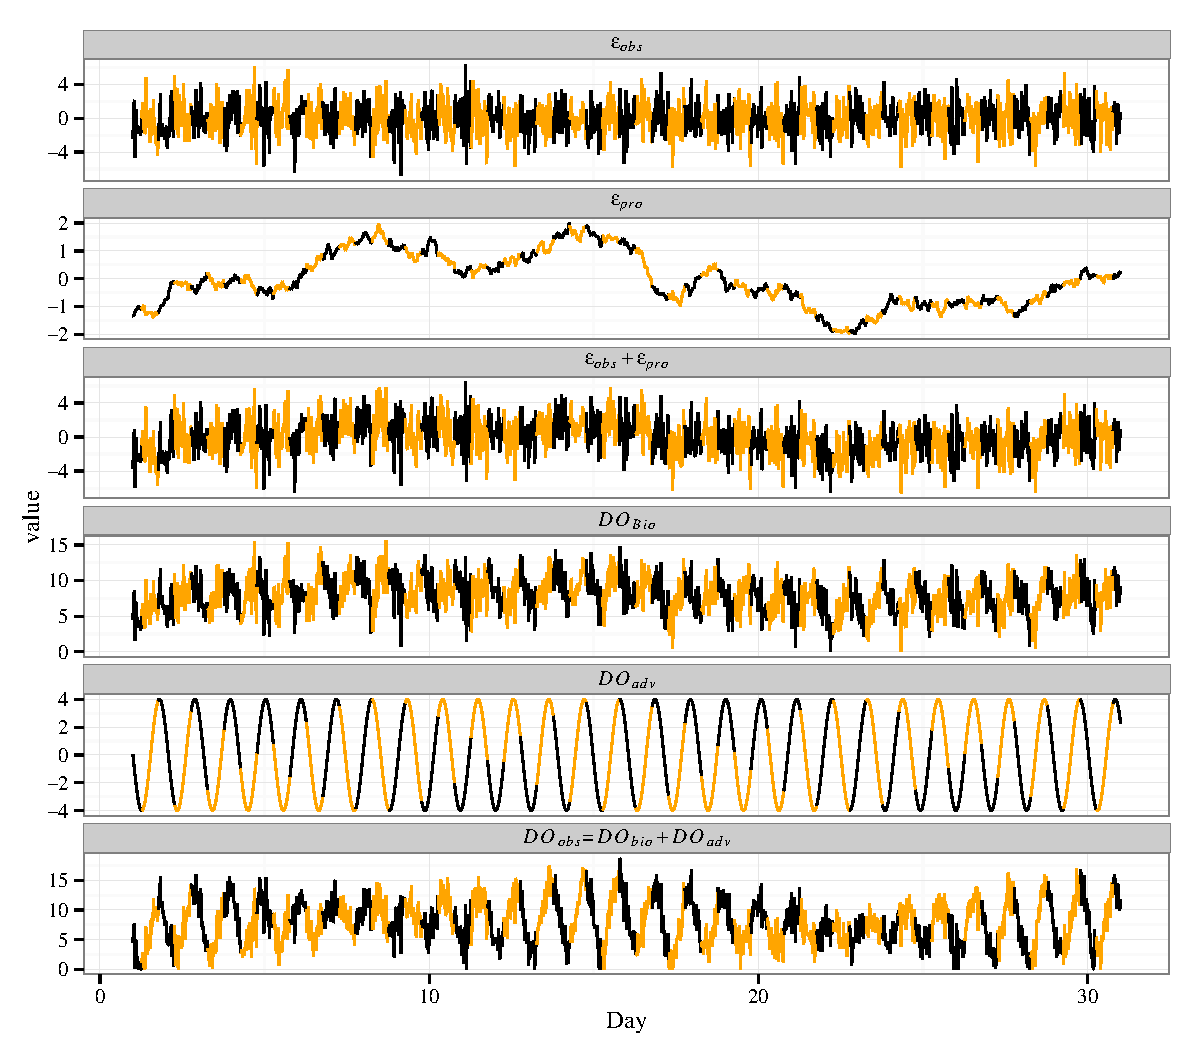
\includegraphics[width=\maxwidth]{figure/do_sim} 

}

\caption[Example of a simulated time series using the equations above]{Example of a simulated time series using the equations above.  Yellow indicates daylight periods.\label{fig:do_sim}}
\end{figure}


\end{knitrout}
\clearpage

% run simulations using eval_grd


% plot of representative time series for simulation
% note that the plot uses data from 'get_prdnrm'  chunk below
\begin{knitrout}
\definecolor{shadecolor}{rgb}{0.969, 0.969, 0.969}\color{fgcolor}\begin{figure}[!h]


{\centering 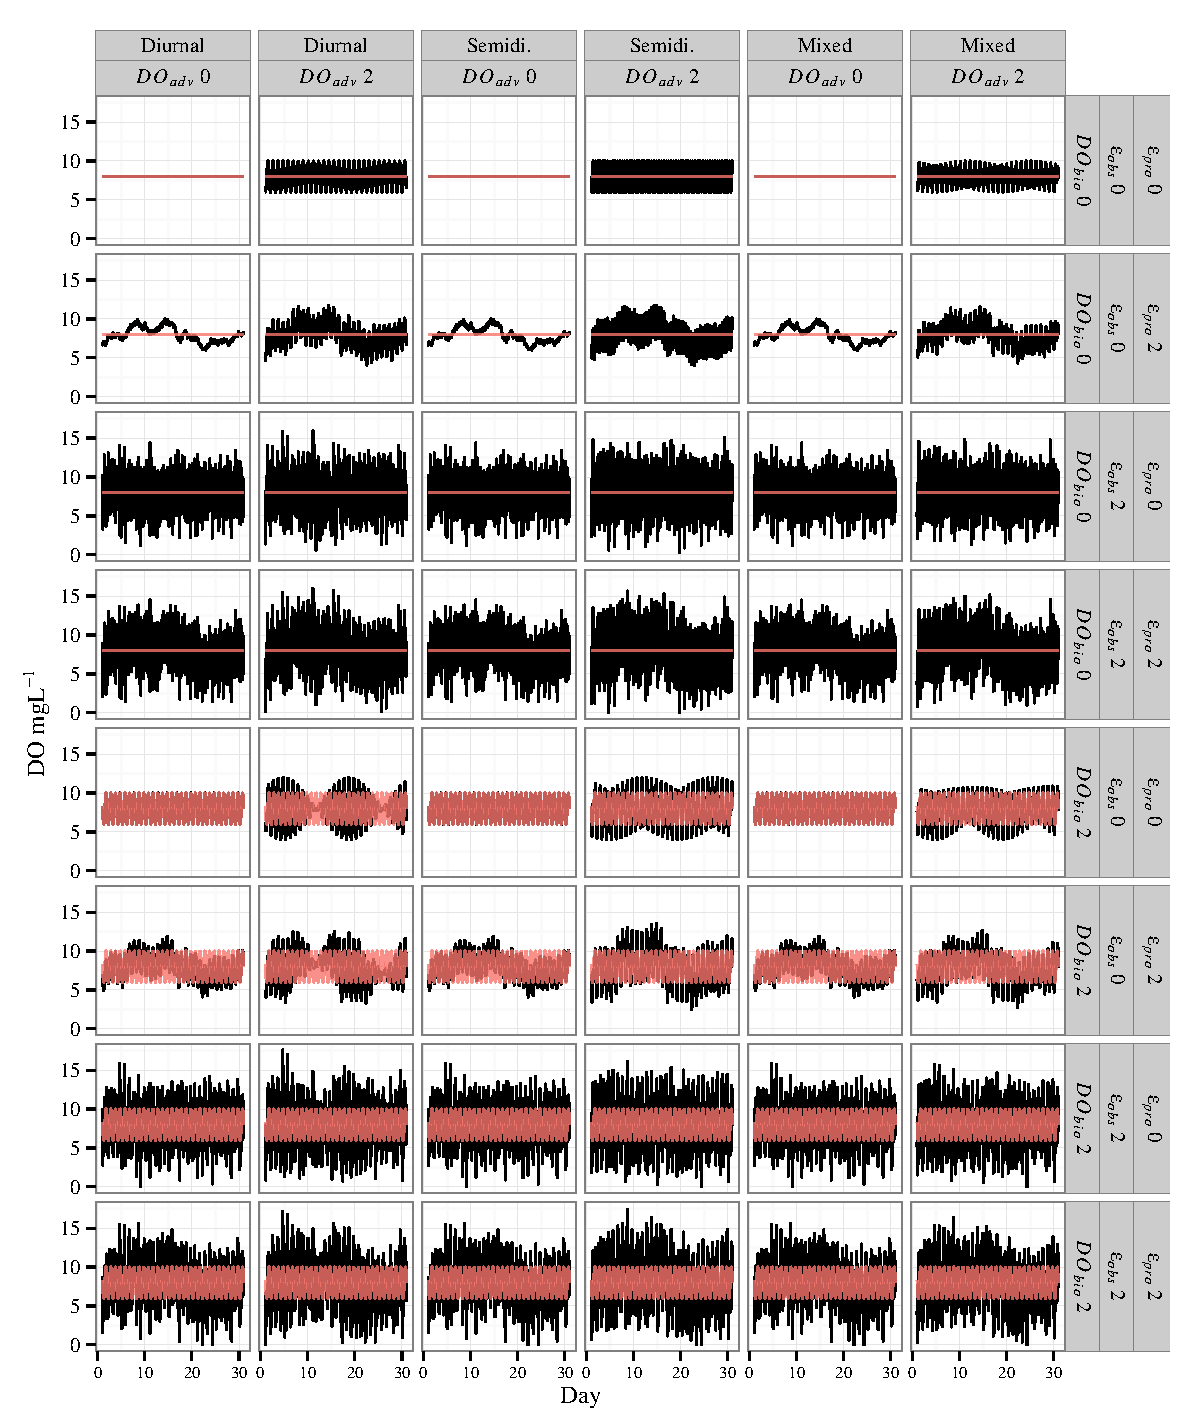
\includegraphics[width=\maxwidth]{figure/sim_ex} 

}

\caption[Representative examples of simulated DO time series]{Representative examples of simulated DO time series.  Black lines are observed DO and red lines are biological DO.\label{fig:sim_ex}}
\end{figure}


\end{knitrout}
\clearpage

% correlation surface for simulation results
\begin{knitrout}
\definecolor{shadecolor}{rgb}{0.969, 0.969, 0.969}\color{fgcolor}\begin{figure}[!h]


{\centering 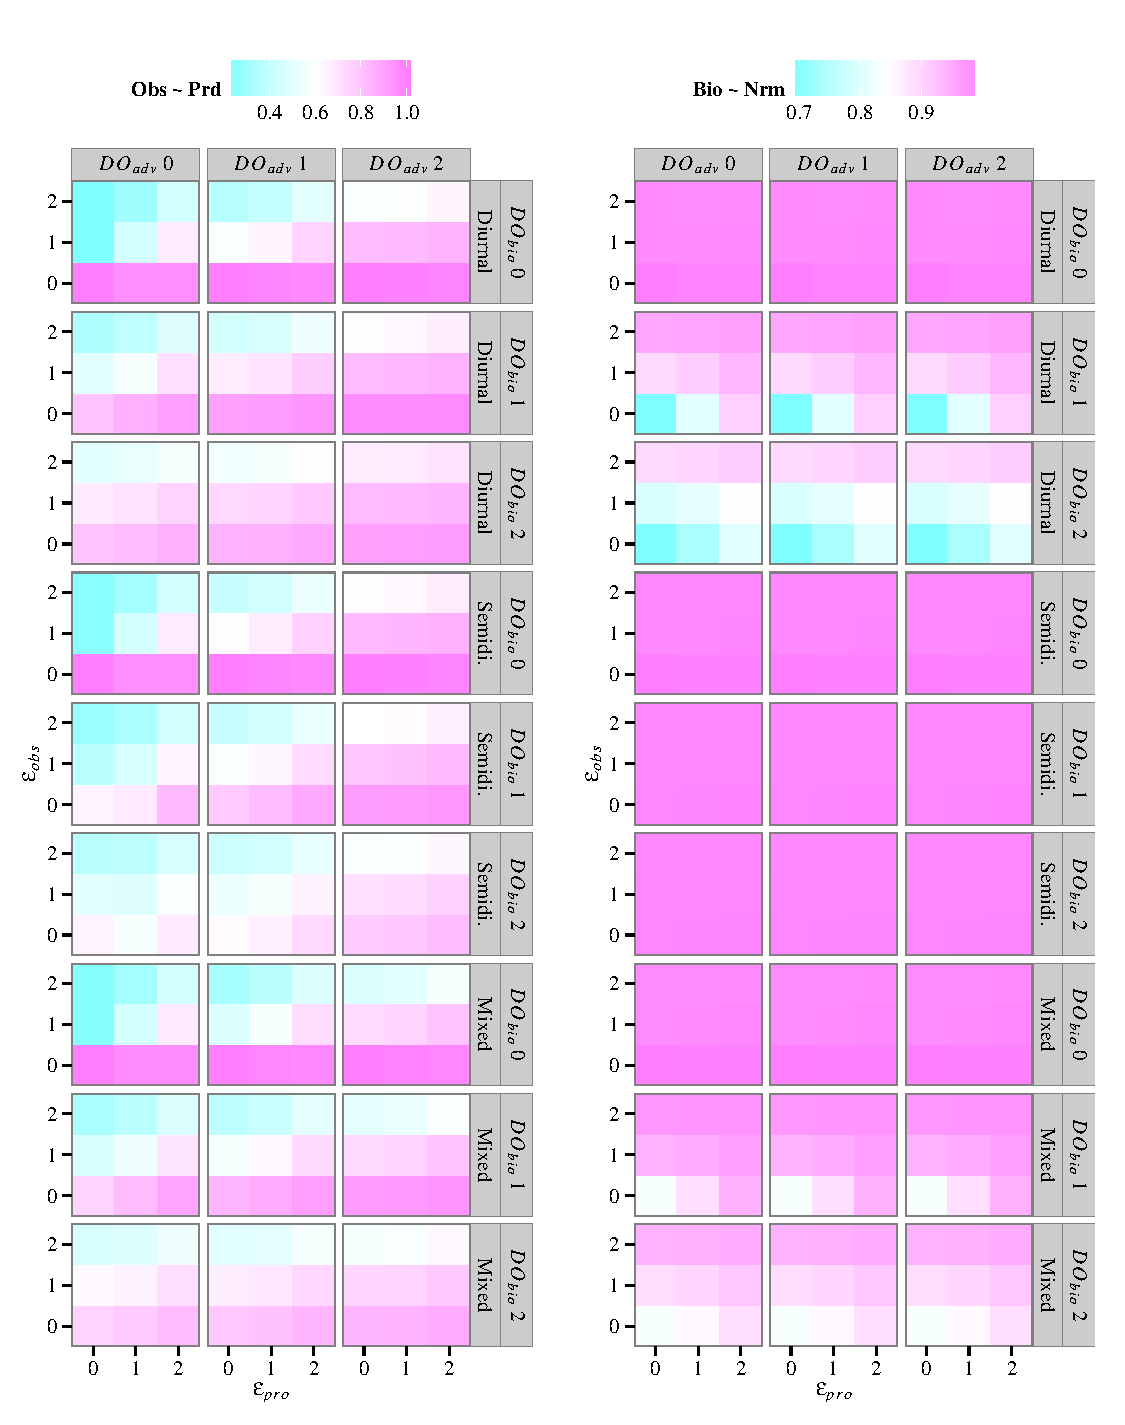
\includegraphics[width=\maxwidth]{figure/cor_surf} 

}

\caption[Correlation surfaces for each unique combination of simulation parameters]{Correlation surfaces for each unique combination of simulation parameters.  The top plots indicate correlations between observed and predicted DO and the bottom plots indicate correlations between biological and normalized DO.\label{fig:cor_surf}}
\end{figure}


\end{knitrout}
\clearpage

% example of creating simulated time series using actual predicted tide

% do simulations with actual tidal data, no figure

\clearpage

\vfill
% get preds, norms from all int_grds w/ actual tidal data, no figure

% correlation surface for simulation results w/ actual tidal data

\vfill
\clearpage

\end{document}
